\documentclass[lettersize,journal]{IEEEtran}
\usepackage{amsmath,amsfonts}
\usepackage{algorithmic}
\usepackage{algorithm}
\usepackage{array}
\usepackage[caption=false,font=normalsize,labelfont=sf,textfont=sf]{subfig}
\usepackage{textcomp}
\usepackage{stfloats}
\usepackage{url}
\usepackage{verbatim}
\usepackage{graphicx}
\usepackage{cite}
\usepackage{xcolor}
\usepackage{parskip}
\usepackage{amsthm}
\hyphenation{op-tical net-works semi-conduc-tor IEEE-Xplore}
% updated with editorial comments 8/9/2021

\begin{document}

\title{An investigation into the effectiveness and impact of a Continuous Delivery pipeline upon university-level games development teams}

\author{Frost Donovan}

\maketitle

\begin{abstract}
    % What's the problem? What am I looking at? How does that help solve the problem? 
    % Opening, Challenge, Action, Resolution 

    Continuous Delivery (CD) is a technique designed to increase reliability and consistency with delivery of builds. This can then help to increase frequency of testing, the accountability of the development team, as well as the teams transpareny and \textit{"all being on the same page ness"}. This can increase team moral as well as stakeholder confidence, as both are able to regularly see the current state and rate of progress for the project. This encourages regular analysis of development pace and project scope, both internal and external. \\
    This stakeholder confidence and awareness of scope is a common problem within student development teams, so this investigation will answer to what extent the deployment of a CD pipeline will help to reduce these problems.
\end{abstract}

\section{Introduction}
    \subsection{What is Continuous Delivery?}
        CD is an expansion of Continuous Integration (CI), a pipeline for the continuous integration of code, being developed on separate branches, into the main branch. This code is merged into the main branch and then tested to ensure there are no merge conflicts or obvious errors thrown from the combined code. Assuming all of these tests pass, this merged code is pushed to the project repository. A key part of this pipeline is that the entire process is automated, ensuring minimal time is wasted waiting for tests to run or code to be uploaded. \cite{ContDelIntro,CICDCD} \\
        CD takes this one step further, in that after a project passes through the CI pipeline, the code is then compiled, packaged, and further tests that require the project to be compiled can be run. These tests should not be run before other tests that don't require compilation due to Fail Fast principles \cite{shore2004fail,bamboo}. Assuming there are no failures during compilation or testing, the built program can then be uploaded to somewhere where it can be easily accessed. Here, it is important to make a distinction between Continuous Delivery, where the build is available internally but not to users, and Continuous Deployment, where the build is pushed straight out to the current product users.
        core to agile methodology \cite{agilemanifesto}

    \subsection{Benefits \& Drawbacks of CD}
        The primary benefit of CD is reduced cycle time - a reduction in the time it takes for a change in the project to happen and then for the user to have that change applied to their version of the software. This principle is core to the agile methodology, being the very first principle in the agile manifesto \cite{agilemanifesto}. This faster cycle time means that feedback from active users can be obtained much quicker, both on the effectiveness of bug fixes and also on new features. Agile is designed to avoid the pitfalls of Waterfall \cite{royce1987managing}, one of which is the commitment of significant time and/ or resources into features that either are unattainable, or not actually wanted by the user. While other agile methods, such as Scrum or Extreme Programming \cite{cohen2004introduction,agilewithscrum}, can be an important part of the agile process, the effectiveness of a development team in delivering \textit{value} is always going to be dependant on the speed and reliability with which user feedback can be obtained. \\
        A benefit of this fast cycle time is not only are players able to see these changes faster, but stakeholders and publishers are able to see development progress, both regularly and on demand. This can be a significant step to building trust between a development studio and publisher, especially if the studio is new or doesn't have an existing relationship with the publisher \cite{gamedevhandbook}. 

        Part of the CD pipeline is testing, with a suite of unit tests being run on the code as part of the build process. As this build process is run consistently, rather than all at once leading up to a main release, this means bugs are found incrementally, stopping the accumulation of technical debt, reducing the cost to fix bugs, and reducing stress on programmers by preventing an overwhelming influx of bugs. While these unit tests will likely catch a lot of bugs, some bugs will only be caught during human playtesting. This decreased cycle time means that human playtesting can happen sooner \& more regularly, and fixes are delivered to testers \& players almost immediately, rather than having to wait for the next release window.
        
        Another strength of a Continuous Delivery pipeline is that it is fully automated. This allows less developer time to be spent setting up build or test environments and manually going through the build process, and more time on actually creating the product. This can be a \textit{significant} time save, with some large scale projects reportedly taking weeks to set up environments ready to produce a release build \cite{paddy, ContDelIntro}. This system also significantly reduces the chance that there are any errors caused by mistakes during the build process as this build-release pipeline will have had many iterations of the product pass through it, before a major release deadline. This increases the reliability and stability of new releases.
    
\section{Background \& Supporting Literature}
    With these benefits in mind it raises two questions; If a CD pipeline is this important and valuable, is it being taught to new developers in further education? If it is, is it actually as effective in practice with student teams as it is in theory?

    There is limited literature relating to Continuous Delivery being implemented in an academic context, and \textit{no} literature that I could find of this being implemented in a game development context. Even upon reviewing a literature review on rapid releases \cite{mantyla2015rapid} there were \textit{no} references to this within a games development context. This lack of literature provides a problem when attempting to find evidence on the performance of CD pipelines, however does highlight a \textit{need} for further literature and case studies on the subject. There is even a lack of literature relating to the effectiveness of CD pipelines within an industry setting. 
    
    Relating to the effect of CD pipeline deployment in an industry setting, a literature review by M{\"a}ntyl{\"a} et al. \cite{mantyla2015rapid} carried out an investigation into firefox's transition "from a TR [Traditional Release] model of one release a year to an RR [Rapid Release] model where new releases come every 6 weeks" \cite[pg 2]{mantyla2015rapid}. This paper concluded that, while there are are many benefits of rapid releases in literature, in this case study the transition from traditional release to a rapid release process "[has] not significantly impacted the product quality" \cite[pg 40]{mantyla2015rapid}. It is worth noting however, that this conclusion has been drawn from an interview with a single Mozilla Firefox QA engineer, as well as the test execution data from 06/2006 to 06/2012. While this data allows a quantitative analysis of the number of tests run or bugs found, it neglects the qualitative side of quality testing, the user's opinion of the software, usability, and perceived work being put into the software. As such, while this case study can give insight into the quantitative effects, it has insufficient evidence to state that the "quality" of the product has not changed \cite{kan2003metrics}.

    

    Given this lack, the papers being reviewed will be based around CD implementation in the academic setting of software development, a parallel field, but one which notably consists much more heavily of code, rather than the more even mix of skills and disciplines that is present within a game development context. As such, these papers all have a lack of analysis on how developers other than programmers respond to a CD pipeline, another case where there is a clear need for further study and literature.


    Has this been done before in academic setting\cite{CDCourse2014,CDMobileDev,IndustryAcademyDenmark}? 
    Links to other things - CI\cite{CICDCD}, Unit tests, regular product reviews, stakeholder (supervisor) confidence, git flow \cite{gitBranching}
    Best practices\cite{duvall2007continuous}? 

\section{Research Question}
    From the above sources, there is a clear need for research into the practical effects of a Continuous Delivery pipeline within game development and game development education. From this knowledge, I propose this initial investigation into the effects of a Continuous Delivery pipeline upon university-level games development teams, with a focus on the confidence of the team, as well as the confidence of the team's academic supervisor in their team. 
    This is purposefully broad, with the aim of encouraging and supporting further research into the topic. Given this, the following hypothesises will be investigated.

    \begin{enumerate}
        \item The use of a CD pipeline will increase a supervisors confidence in their team's ability to deliver a new, working build each week. (Q.S1)
        \item The team's confidence and the supervisors confidence in being able to achieve everything within the scope of the project will be much more closely related with the use of a CD pipeline.(Q.S2,St1 plotted against time)
        \item A CD pipeline will help developers understand the current state of the project (Q.St2)
        \item A CD pipeline will help developers to always know why the work they are doing is being done (Q.St3)
        \item A team using a CD pipeline will refine their scope more often (Q.St4)
        \item A team using a CD pipeline will do more playtesting
    \end{enumerate}

\section{Research Methodology}
    \subsection{Experimental Design}
        

    \subsection{Limitations}
        The primary limitation in this study is time. If this study were to be expanded, I would ideally like to follow team's from their first year all the way through to graduation, introducing half of the teams to the CD pipeline immediately and then tracking their results, feedback, and attitudes across all three years against the control groups. This could also be done across multiple cohorts, providing increased statistical significance and helping to account for random variation within team's cohesion and skill level. I could also foresee a technical and potentially ethical problem with this approach however.
        
        Technically, within Falmouth University Game's Academy, the department where these studies have taken place, teams are not the same each year, they are randomised. This would mean it would be impossible to track the same 'team', although potentially individuals could be tracked and seeing if they implemented CD pipelines of their own accord in future teams could also be a revealing statistic to look at, as it would likely give a measure of \textit{perceived} value, rather than actual value. \\
        The potential ethical problem could be if the initial results point towards a CD pipeline effecting a students grade, how is that dealt with. Does the experiment carry on as planned, potentially wilfully disadvantaging particular groups of students? While I am uncertain if this would be considered an ethical problem by an ethics board, it could likely provide a moral problem for those involved in running the study. A potential solution could be that those running the experiment would have to be kept in the dark about it's results while it was ongoing to prevent and bias or conflict of interest. While this would certainly require due consideration, it is not a concern for this initial study.

        Another limitation is that of resources available. Ideally, every team which a CD pipeline deployed would have support to help customise the pipeline, supporting the team in building custom processes and writing robust unit tests. This would likely give the most 'accurate' imitation of a CD pipeline under industry conditions, however we are unable to provide that level of support due to the research team being a singular individual whom has other commitments, and also lacks the experience to guide teams in writing unit tests specifically.

    \subsection{Sampling}
        Random sampling within Falmouth University Games Academy game's development teams. Aim is to sample as much of the population as possible, including team's across all three years. Mix of random and convenience sampling - any team within the GA is eligible, but will mostly be recruiting teams by speaking to teams in the ga as that's the easiest way to communicate. Will likely also get email sent to all students asking them to participate. \\
        Population is split into four substrata, first years, second years, third years, masters students. Participant teams will then be evenly split between experimental groups who will be given the CD pipeline and control groups. which team's are control groups will be random. This random gathering of participants and assigning of control groups is purposefully to help account for random variation in team skill and cohesion across all potential participant teams.

        Data will initially be treated as a single strata, even numbers across each substrata will be to potentially allow for further analysis on if CD effect vary by year.

        Critical size for statistical significance?
    
    \subsection{Data management plan}
        Data shall be collected using Microsoft Forms as it is GDPR compliant out the box. It will then be stored using Microsoft One Drive, another application that is GDPR compliant out the box.
        Data will be anonymised but matched after it has been collected, with participants names matching to unique ID numbers. The data will then be stored with this ID, rather than anything identifying like a name or email.
    
    \subsection{Data Analysis}
        only one result pre-test while ~10 results post-test
        Not enough data pre-test to make meaningful conclusions?
        state of project is not comparative

        study is initial investigation - could run matched pairs \& try and test all H's but then talk about the lack of pre-test data and that these things would likely change as  project progress's and a team move's through stages of team forming \textbf{cite for team forming stages}, so results may be indicative but not conclusive. Could provide a base for further research but not to be taken without consideration of limitations 
        Could introduce CD pipeline later? Gather pre-test data up to the end of Feb (4 feedbacks), then implement pipeline first week of march, and then gather post-test data up to end of March (4 feedbacks)
        sample size for matched is 34 - 34 \textit{groups} would be around 2/3 the GA at a rough guess.. potentially doable, would need to run first form week starting Jan 10th so could gather as many groups as possible up to then and then decide? Have two plans dependant on the number of participants I can secure. If I can secure 34 groups would get H's based on individuals to Power of 0.9999969 assuming 5 people per group respond to survey which would likely low
        Could use ANOVA w/ repeated measurements between factors. One group has CD pipeline one is control group - two groups are independent (it's different teams in each group) so it is between factors not within factors test \url{https://carvadia.com/what-is-the-difference-between-a-within-subjects-anova-and-a-between-subjects-anova/}. Give's a req sample size of 20 with 8 measures. This would let me run all hypothesises with control \& experiment group! Nice! michaels advice was to use f of 0.4 as that is Cohen's recommended value (https://www2.psych.ubc.ca/~schaller/528Readings/Cohen1992.pdf)
        http://www.mormonsandscience.com/gpower-guide.html

        \begin{figure}[h!]
            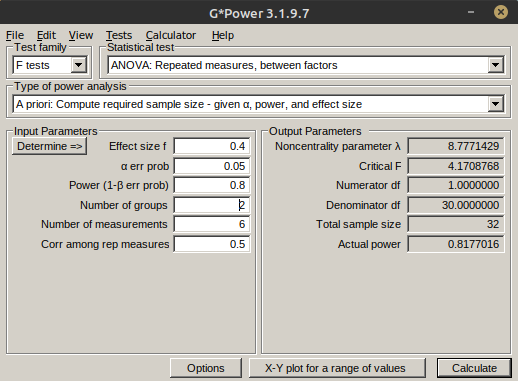
\includegraphics[width=0.5\textwidth]{Images/ANOVA_2.png}
            \caption{Screen capture from GPower software showing sample size caluclation for a two tailed, matched pair t test}
            \label{ANOVArepeatedbetween}
        \end{figure}

        \textit{The use of a CD pipeline will increase a supervisors confidence in their team's ability to deliver a new, working build each week.} \\
            Q.S1
            matched pair
            Sample size is in groups
            t-test
            two tailed as we care about if it reduces the supervisors confidence as that would be bad
            80\% Power
            Total sample size is likely too high to be feasible
            \begin{figure}[h!]
                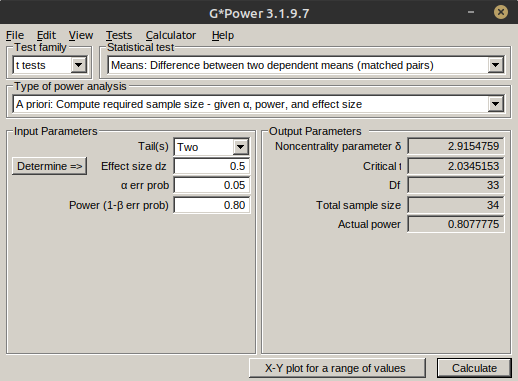
\includegraphics[width=0.5\textwidth]{Images/GPower_Matched.png}
                \caption{Screen capture from GPower software showing sample size caluclation for a two tailed, matched pair t test}
                \label{twotailmatchedpair}
            \end{figure}

        \textit{The team's confidence and the supervisors confidence in being able to achieve everything within the scope of the project will be more closely related with the use of a CD pipeline} \\
            Q.S2 \& Q.St1 plotted against time
            independent, matched pairs wouldn't work as this confidence \& the scope will change as the project progresses and the amount of time left decreases \& it becomes easier to estimate. Although this becomes easier for the team \& the supervisor.
            Could potentially do matched pairs
            sample size is in groups
            take average difference each month, compare experimental against control group
            \begin{figure}[h!]
                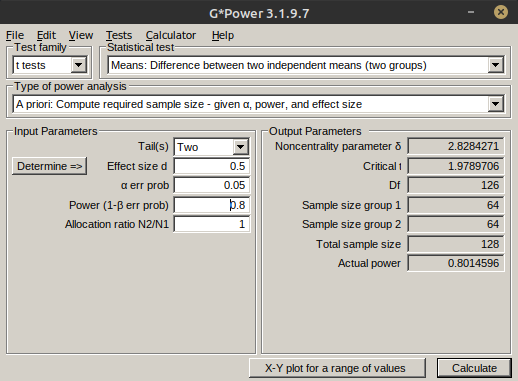
\includegraphics[width=0.5\textwidth]{Images/GPower_Independent.png}
                \caption{Screen capture from GPower software showing sample size caluclation for H2}
                \label{twotailindependent}
            \end{figure}

        \textit{A CD pipeline will help developers understand the current state of the project} \\
            Q.St2
            two tailed, matched pair
            sample size is individual not group
            compare pre test to post test at start, mid, and end
            not convinced I'll be able to say with confidence using matched pair due to lack of pre-test data
            see figure \ref{twotailmatchedpair}

            Could do two independent groups
            much more meaningful data at getting a more true comparison
            sample size is \textit{potentially} do able
            see figure \ref{twotailindependent}


        \textit{A CD pipeline will help developers to always know why the work they are doing is being done} \\
            Q.St3
            sample size is individual not group
            potentially feasible to run independent groups
            see figure \ref{twotailindependent}

        \textit{A team using a CD pipeline will refine their scope more often} \\
            Q.St4
            sample size is group not individual
            likely not feasible

            see figure \ref{twotailindependent}

        \textit{A team using a CD pipeline will do more playtesting} \\
            Q.St5
            sample size is group not individual
            independent as the state of the project will change so playtesting priority will not be constant
            see figure \ref{twotailindependent}
    
        Two sample t-test as we are looking for difference between two groups (those with CD \& those without)
        different tests for each hypothesis
        T-test? Critical size for statistical significance?
        $\alpha$ error probability should stay at 5 \%
        $\beta$ error probability has much more flexibility, could reasonably push as low as 80\%
        pre-test vs post-test could use t test two tailed means difference between two dependant OR F test ANCOVA
        could potentailly use T test w/ two independent groups for student values due to sample size, supervisor data would need to be matched pairs due to required sample size

        justify effect size - 0.5 is reasonable but need to justify. "only large effects have practical relevance so making test sensitive to large effects"

    \subsection{Ethical Considerations}
        Due to the nature of this research, there are minimal ethical considerations that need to be taken into account. The participants will not be exposed to any potential risks outside of what they would experience under normal circumstances, although an effort has been made to keep the feedback form fairly condensed. This is to minimise any increased stress that the commitment of having to fill out the form may cause.
    
    \section{Appendix}
    Data analysis code, supporting screenshots, list of unit tests \& testing plan

\section{Artifact}
    briefly describe artifact
    make a brief note on quality assurance
    link to git repo
    show off any screenshots or code excerpts

    More interested in what and how at this stage

    two repo link - one with artifact to easily show off then give link to show it embedded in main project
    \subsection{What will be made}
        CD pipeline utilising Github Actions. Tool to set up secrets? Would be sick \url{https://docs.github.com/en/rest/reference/actions#secrets} \\
        Continuous delivery or continuous deployment? Scope as deployment would need to include itch integration w/ butler, although it looks relatively simple to set up.
        Auto-upload to steam \& itch! \url{https://itch.io/docs/butler/}

    \subsection{How will I ensure Quality}
        Quality control. Roadmap? Unit Testing? Integration testing?

    \subsection{How will I create it}

    \subsection{Why will this answer the questions}

\bibliographystyle{ieeetr}
\bibliography{bibliography}

\end{document}